\documentclass[12pt,a4paper]{article}

% ===== PACKAGES =====
\usepackage[utf8]{inputenc}
\usepackage[T1]{fontenc}
\usepackage[french]{babel}
\usepackage{geometry}
\usepackage{setspace}
\usepackage{titlesec}
\usepackage{fancyhdr}
\usepackage{graphicx}
\usepackage{amsmath}
\usepackage{amssymb}
\usepackage{hyperref}
\usepackage{xcolor}
\usepackage{enumitem}
% \usepackage{microtype}
\usepackage{booktabs}
\usepackage{mdframed}
\usepackage{parskip}

% ===== MISE EN PAGE =====
\geometry{
  headheight=15pt,
  a4paper,
  top=2.5cm,
  bottom=2.5cm,
  left=3cm,
  right=2.5cm
}

% ===== COULEURS =====
\definecolor{navyblue}{RGB}{0, 51, 102}
\definecolor{lightgray}{RGB}{245, 245, 245}
\definecolor{accentblue}{RGB}{0, 102, 179}

% ===== INTERLIGNE =====
\setstretch{1.3}

% ===== HYPERLIENS =====
\hypersetup{
  colorlinks=true,
  linkcolor=navyblue,
  citecolor=navyblue,
  urlcolor=accentblue,
  pdftitle={Rapport d'avancement de memoire de Master 2},
  pdfauthor={TSAFACK NTEUDEM Erick}
}

% ===== EN-TETE ET PIED DE PAGE =====
\pagestyle{fancy}
\fancyhf{}
\fancyhead[L]{\small\textcolor{navyblue}{Rapport de Master -- TSAFACK NTEUDEM Erick}}
\fancyhead[R]{\small\textcolor{navyblue}{\thepage}}
\fancyfoot[C]{\small\textcolor{gray}{Universit\'e de Dschang -- Ann\'ee Acad\'emique 2025/2026}}
\renewcommand{\headrulewidth}{0.5pt}
\renewcommand{\footrulewidth}{0.5pt}

% ===== FORMAT DES TITRES =====
\titleformat{\section}
  {\large\bfseries\color{navyblue}}
  {\Roman{section}.}{0.5em}{}
  [\vspace{-0.3em}\rule{\linewidth}{0.5pt}\vspace{0.3em}]

\titleformat{\subsection}
  {\normalsize\bfseries\color{navyblue}}
  {\thesubsection}{0.5em}{}

\titlespacing{\section}{0pt}{1.2em}{0.6em}
\titlespacing{\subsection}{0pt}{0.8em}{0.4em}

% ===== LISTES =====
\setlist[itemize]{leftmargin=1.5em, itemsep=0.2em, parsep=0pt, topsep=0.4em}
\setlist[enumerate]{leftmargin=1.5em, itemsep=0.2em, parsep=0pt, topsep=0.4em}

% ===== ENCADRE POUR QUESTION DE RECHERCHE =====
\newmdenv[
  backgroundcolor=lightgray,
  linecolor=navyblue,
  linewidth=1.5pt,
  leftline=true,
  rightline=false,
  topline=false,
  bottomline=false,
  innerleftmargin=12pt,
  innerrightmargin=8pt,
  innertopmargin=8pt,
  innerbottommargin=8pt
]{questionbox}

% ===== DEBUT DU DOCUMENT =====
\begin{document}

% ===== PAGE DE COUVERTURE =====
\begin{titlepage}
\thispagestyle{empty}
\begin{center}

\vspace*{0.5cm}
{\Large\bfseries\color{navyblue} UNIVERSIT\'E DE DSCHANG}\\[0.3cm]
{\normalsize Facult\'e des Sciences}\\[0.1cm]
{\normalsize D\'epartement de Math\'ematiques et Informatique}\\[0.1cm]
{\small\itshape Unit\'e de Recherche en Informatique Fondamentale, Ing\'enieries et Applications (URIFIA)}

\vspace{1.5cm}
\rule{\linewidth}{1.5pt}\\[0.4cm]
{\Large\bfseries\color{navyblue} RAPPORT D'AVANCEMENT DE M\'EMOIRE DE MASTER 2}\\[0.4cm]
\rule{\linewidth}{1.5pt}

\vspace{1.2cm}
{\Large\bfseries
Une approche d'explicabilit\'e des mod\`eles d'apprentissage profond\\[0.3cm]
pour le contr\^ole d'acc\`es aux donn\'ees et aux traitements :\\[0.3cm]
\textit{Les Self-Interpretable Neural Networks}}

\vspace{2cm}
\begin{minipage}{0.48\textwidth}
  \begin{flushleft}
    \textbf{R\'edig\'e par :}\\[0.2cm]
    TSAFACK NTEUDEM Erick\\
    \textit{Matricule : CM-UDS-23SCI1383}
  \end{flushleft}
\end{minipage}
\hfill
\begin{minipage}{0.48\textwidth}
  \begin{flushright}
    \textbf{Sous la supervision de :}\\[0.2cm]
    Dr. AZANGUEZET QUIMATIO\\
    Benoît Martin\\
    \textit{Charg\'e de cours, Universit\'e de Dschang}
  \end{flushright}
\end{minipage}

\vfill
{\normalsize Ann\'ee Acad\'emique : 2025/2026}

\end{center}
\end{titlepage}

% ===== TABLE DES MATIERES =====
\newpage
\tableofcontents
\newpage

% ===================================================================
% I. CONTEXTE ET MOTIVATION
% ===================================================================
\section{Contexte et Motivation}

L'essor des mod\`eles d'apprentissage profond (\textit{deep learning}) a r\'evolutionn\'e de nombreux domaines, notamment la cybers\'ecurit\'e, o\`u ils sont de plus en plus employ\'es pour le contr\^ole d'acc\`es aux donn\'ees. Cette t\^ache exige transparence et justification afin d'assurer la s\'ecurit\'e et la conformit\'e r\'eglementaire. Les mod\`eles de deep learning, bien qu'efficaces pour traiter des donn\'ees complexes, souffrent d'une opacit\'e qualifi\'ee de \textit{bo\^ite noire}, freinant leur adoption dans des contextes critiques o\`u la responsabilit\'e et la confiance sont primordiales.

Les approches classiques de contr\^ole d'acc\`es telles que le DAC (\textit{Discretionary Access Control}), le MAC (\textit{Mandatory Access Control}), le RBAC (\textit{Role-Based Access Control}) \cite{sandhu1996}, le Or-BAC (\textit{Organization-Based Access Control}) et le HOr-BAC (\textit{Hierarchical Organization-Based Access Control}) \cite{azanguezet2016} reposent sur des r\`egles pr\'ed\'efinies offrant une transparence naturelle mais une adaptabilit\'e limit\'ee face aux environnements dynamiques tels que les syst\`emes IoT ou le cloud. Ces mod\`eles n\'ecessitent une ing\'enierie manuelle co\^uteuse d'attributs et de politiques \cite{nobi2022}, ce qui les rend sujets aux erreurs humaines (\textit{sur-provisionnement} ou \textit{sous-provisionnement}) et difficiles \`a maintenir \`a grande \'echelle.

En revanche, les mod\`eles d'apprentissage profond permettent une analyse en temps r\'eel des acc\`es gr\^ace \`a leur capacit\'e d'adaptation. Toutefois, leur adoption est entrav\'ee par leur opacit\'e, rendant difficile l'audit et la justification des d\'ecisions. Dans ce cadre, les r\'eglementations comme le R\`eglement G\'en\'eral sur la Protection des Donn\'ees (RGPD) exigent une explicabilit\'e stricte : l'article~22 stipule le droit \`a une explication des d\'ecisions automatis\'ees. Cette contrainte met en lumi\`ere l'urgence de d\'evelopper des m\'ethodes d'intelligence artificielle explicable (XAI) capables de concilier performance et transparence\cite{goodman2017}.

Les approches post-hoc, telles que LIME et SHAP, offrent des solutions partielles pour pallier ce manque d'interpr\'etabilit\'e, mais pr\'esentent des limites importantes en termes de robustesse \cite{rudin2019}: elles sont fragiles face aux attaques adversariales, peu fid\`eles au v\'eritable fonctionnement du r\'eseau, instables pour des entr\'ees similaires, et computationnellement co\^uteuses \cite{slack2020}. Dans un syst\`eme de d\'ecision critique comme le contr\^ole d'acc\`es, ces limites peuvent engendrer une fausse confiance dans les d\'ecisions rendues.

Les r\'eseaux neuronaux auto-interpr\'etables (SINN \textit{Self-Interpretable Neural Networks}) se positionnent comme une r\'eponse prometteuse \`a ces d\'efis, en int\'egrant l'interpr\'etabilit\'e intrins\`eque directement dans l'architecture du mod\`ele, sans compromettre l'efficacit\'e des pr\'edictions. C'est dans ce contexte que s'inscrit le pr\'esent travail de recherche.

% ===================================================================
% II. PROBLEMATIQUE
% ===================================================================
\section{Probl\'ematique}

Les syst\`emes de contr\^ole d'acc\`es bas\'es sur le deep learning pr\'esentent une triple tension : ils sont performants mais opaques, efficaces mais non conformes aux exigences r\'eglementaires, et pr\'ecis mais difficilement auditables. Cette situation soul\`eve la question de recherche centrale suivante :

\begin{questionbox}
\textit{Comment d\'evelopper une m\'ethode d'explicabilit\'e pour les mod\`eles d'apprentissage profond utilis\'es dans le contr\^ole d'acc\`es, assurant la fid\'elit\'e des explications aux pr\'edictions tout en r\'epondant aux enjeux d'opacit\'e, de biais et de conformit\'e r\'eglementaire~?}
\end{questionbox}

Trois obstacles principaux emp\^echent l'adoption des mod\`eles de deep learning dans le contr\^ole d'acc\`es :

\begin{itemize}
  \item L'opacit\'e des d\'ecisions, rendant difficile l'audit et la justification des refus ou autorisations d'acc\`es ;
  \item Les exigences r\'eglementaires, n\'ecessitant des explications conformes au RGPD et auditables par des autorit\'es comp\'etentes ;
  \item Les risques de biais dans les donn\'ees, pouvant entra\^iner des d\'ecisions in\'equitables et discriminatoires.
\end{itemize}

Ces contraintes mettent en \'evidence le besoin urgent d'une architecture de contr\^ole d'acc\`es bas\'ee sur le deep learning qui soit \`a la fois performante, transparente et actionnable. Le type d'explication id\'eal pour ce domaine est double : des explications sous forme de \textbf{r\`egles logiques} (globales et auditables) et des \textbf{explications contrefactuelles} (locales et actionnables), r\'epondant \`a la question ``Que faut-il modifier pour obtenir ou refuser un acc\`es~?''.

% ===================================================================
% III. OBJECTIFS
% ===================================================================
\section{Objectif Principal et Objectifs Sp\'ecifiques}

\subsection{Objectif principal}

L'objectif principal de ce travail est de concevoir un mod\`ele d'apprentissage profond unifi\'e pour le contr\^ole d'acc\`es aux donn\'ees et aux traitements, capable de produire simultan\'ement des d\'ecisions pr\'ecises et des explications interpr\'etables, tant sous forme de r\`egles logiques auditables que de contrefactuels actionnables en un seul passage avant (\textit{single forward pass}).

\subsection{Objectifs sp\'ecifiques}

\begin{enumerate}
  \item \textbf{Collecter et pr\'etraiter les donn\'ees pertinentes} : adapter le jeu de donn\'ees Amazon, utilis\'e dans les travaux de DLBAC, pour refl\'eter des sc\'enarios r\'ealistes de contr\^ole d'acc\`es, en \'eliminant les bruits et en extrayant les caract\'eristiques pertinentes ;

  \item \textbf{Explorer et analyser les m\'ethodes existantes} : \'etudier la compatibilit\'e des approches actuelles (DLBAC, HyConEx, HyperLogic) avec les exigences du contr\^ole d'acc\`es, en identifiant leurs forces et leurs limites respectives ;

  \item \textbf{Concevoir un mod\`ele unifi\'e (RuleConEx)} : int\'egrer dans une seule architecture un hypernetwork g\'en\'erateur de r\`egles locales interpr\'etables (inspir\'e de HyperLogic) et un g\'en\'erateur de contrefactuels plausibles (inspir\'e de HyConEx) ;

  \item \textbf{\'Evaluer les performances et l'interpr\'etabilit\'e} : mesurer les performances du mod\`ele propos\'e via des m\'etriques standards (ROC AUC, F1-score, validit\'e des contrefactuels, plausibilit\'e) et les comparer aux approches classiques et aux m\'ethodes de l'\'etat de l'art ;

  \item \textbf{Assurer la conformit\'e r\'eglementaire} : produire des explications lisibles par un humain, conformes aux exigences du RGPD, et exploitables pour l'audit des politiques d'acc\`es.
\end{enumerate}


% ===================================================================
% V. ETAT DE L'ART
% ===================================================================
\section{\'Etat de l'Art}
\label{sec:etat-art}

L'\'etat de l'art de ce travail s'articule autour de trois travaux fondateurs directement li\'es \`a la probl\'ematique : DLBAC, HyConEx et HyperLogic.

\subsection{DLBAC \textit{Deep Learning Based Access Control}}

Nobi et al. (2022)~\cite{nobi2022} ont propos\'e DLBAC, une approche de contr\^ole d'acc\`es fond\'ee sur l'apprentissage profond qui r\'epond aux limites des mod\`eles classiques. L'id\'ee centrale est de remplacer les r\`egles d'acc\`es par un r\'eseau de neurones profond entra\^in\'e directement sur les m\'etadonn\'ees brutes des utilisateurs et des ressources, sans ing\'enierie manuelle d'attributs ni de politiques.

Le prototype DLBAC$_\alpha$ a \'et\'e \'evalu\'e sur deux jeux de donn\'ees r\'eels (dont Amazon) et huit jeux de donn\'ees synth\'etiques de complexit\'e croissante. DLBAC$_\alpha$ surpasse les m\'ethodes de \textit{policy mining} (XuStoller, Rhapsody, EPDE-ML) et les classifieurs ML classiques (RF, SVM, MLP) sur les scores F1, le taux de vrais positifs (TPR), et la g\'en\'eralisation. Il offre un meilleur \'equilibre entre sur-provisionnement et sous-provisionnement, et s'av\`ere plus robuste face \`a la complexit\'e des donn\'ees.

Cependant, DLBAC reste un mod\`ele opaque. Les auteurs proposent des pistes d'explicabilit\'e post-hoc (\textit{Integrated Gradients}, extraction d'arbres de d\'ecision approximatifs), mais celles-ci restent externes et pr\'esentent les limites inh\'erentes \`a toutes les m\'ethodes post-hoc. DLBAC identifie lui-m\^eme l'explicabilit\'e intrins\`eque comme une direction future prioritaire, ce qui constitue pr\'ecis\'ement le c{\oe}ur du pr\'esent travail.

\subsection{HyConEx \textit{Hypernetwork Classifier with Counterfactual Explanations}}

HyConEx~\cite{hyconex2026} est un mod\`ele de classification con\c{c}u pour les donn\'ees tabulaires, qui combine dans une seule architecture une pr\'ediction de classe performante et la g\'en\'eration de contrefactuels plausibles pour toutes les classes alternatives, le tout produit en un seul \textit{forward pass}. Il s'agit de la premi\`ere approche int\'egrant simultan\'ement pr\'ediction et explication contrefactuelle dans un m\^eme mod\`ele.

Le m\'ecanisme central repose sur un hypernetwork $H(x;\theta)$ qui, pour chaque entr\'ee $x$, g\'en\`ere une matrice de poids $W$ d\'efinissant un classifieur lin\'eaire local. Les lignes de cette matrice servent \`a produire des contrefactuels par translation : $x' = x - W_m$. Trois conditions doivent \^etre satisfaites pour chaque contrefactuel : il doit \^etre correctement classifi\'e dans la classe cible, rester proche de l'entr\'ee originale, et \^etre plausible (\textit{in-distribution}), cette derni\`ere condition \'etant assur\'ee par un flux normalisant conditionnel.

Les exp\'eriences montrent que HyConEx atteint des performances comp\'etitives en classification (AUROC jusqu'\`a 0.999 sur certains jeux de donn\'ees) et g\'en\`ere des contrefactuels de qualit\'e comparable aux m\'ethodes externes (PPCEF, CEGP, CEM), tout en \'etant plusieurs ordres de grandeur plus rapide : 0.003 secondes contre plusieurs milliers de secondes pour les m\'ethodes concurrentes. Le mod\`ele g\`ere \'egalement correctement les variables cat\'egorielles gr\^ace \`a un lissage softmax \`a basse temp\'erature.

\subsection{HyperLogic \textit{Enhancing Diversity and Accuracy in Rule Learning with HyperNets}}

HyperLogic~\cite{hyperlogic2024}, pr\'esent\'e \`a NeurIPS~2024 par Yang Yang, Wendi Ren et Shuang Li, est un cadre g\'en\'erique qui int\`egre des hypernetworks dans l'apprentissage diff\'erentiable de r\`egles logiques IF-THEN. L'objectif est d'augmenter la diversit\'e et la pr\'ecision des r\`egles apprises tout en pr\'eservant l'interpr\'etabilit\'e, en contournant les limitations structurelles des r\'eseaux de r\`egles classiques qui sont souvent trop rigides et peu expressifs.

L'hypernetwork de HyperLogic prend comme entr\'ee un bruit gaussien $\varepsilon$ et g\'en\`ere les poids $\theta = G(\varepsilon)$ du r\'eseau principal (inspir\'e de DR-Net). Ce r\'eseau principal est un r\'eseau \`a deux couches : une couche \textit{Rule}, qui apprend des conjonctions logiques via une approximation diff\'erentiable de la fonction indicatrice, et une couche \textit{OR}, qui combine les r\`egles de mani\`ere additive pond\'er\'ee. En une seule session d'entra\^inement, HyperLogic peut g\'en\'erer jusqu'\`a 5\,000 ensembles de r\`egles candidats, parmi lesquels on s\'electionne le meilleur selon des crit\`eres de performance et de concisit\'e.

La r\'egularisation combine deux termes : une divergence KL pour encourager la diversit\'e des ensembles de r\`egles g\'en\'er\'es, et une norme $\ell_1$ pour encourager la sparsit\'e (r\`egles concises) :
\[
\ell_{\text{reg}} = \lambda_1\, D_{\text{KL}}(\mu \,\|\, \mu_0)
+ \lambda_2\, \mathbb{E}_\mu\!\left[\sum_{k=1}^K |u_k|\right]
\]

Les exp\'eriences sur quatre jeux de donn\'ees binaires (\textit{magic}, \textit{adult}, \textit{house}, \textit{heloc}) montrent que HyperLogic am\'eliore les performances de DR-Net et surpasse les m\'ethodes classiques (CG, BRS, RIPPER) en termes de pr\'ecision, tout en r\'eduisant la complexit\'e des r\`egles. L'analyse th\'eorique \'etablit que HyperLogic est un approximateur universel dans l'espace de Barron.



\subsection{Limite de HyConEx et HyperLogic}
Bien que \textbf{HyConEx} excelle dans la génération de contrefactuels locaux actionnables et qu'\textbf{HyperLogic} permette d'apprendre des règles interprétables et diversifiées, aucun des deux modèles ne produit simultanément ces deux types d'explications complémentaires. HyConEx ne génère pas de règles globales auditées, tandis qu'HyperLogic ne fournit pas d'explications contrefactuelles locales. C'est cette limite que notre modèle unifié \textbf{RuleConEx} vise à surmonter en intégrant ces deux approches au sein d'une seule architecture.

% ===================================================================
% IV. OUTILS ET METHODES
% ===================================================================
\section{Outils et M\'ethodes}

\subsection{Donn\'ees}

Les exp\'erimentations s'appuient sur le corpus \textbf{DLBAC} de Nobi et al.~\cite{nobi2022}, disponible dans le d\'ep\^ot \texttt{DlbacAlpha-main}. On distingue :
\begin{itemize}
  \item \textbf{huit jeux synth\'etiques} (\texttt{u4k-r4k-auth11k} \`a \texttt{u6k-r6k-auth32k}) : tuples d'autorisation simul\'es, avec 4 op\'erations d'acc\`es (\texttt{op1}--\texttt{op4}) et des m\'etadonn\'ees utilisateur/ressource de cardinalit\'e variable ;
  \item \textbf{trois jeux Amazon r\'eels} (\texttt{amazon1}, \texttt{amazon2}, \texttt{amazon3}) : historiques d'acc\`es issus des benchmarks Kaggle/UCI, avec d\'ecision binaire \textit{grant}/\textit{deny}.
\end{itemize}
Chaque ligne brute d'un fichier \texttt{.sample} encode un tuple
$\langle uid, rid, m^u_1,\ldots,m^u_i, m^r_1,\ldots,m^r_j, op_1,op_2,op_3,op_4\rangle$.
Le d\'etail du pipeline de transformation est pr\'esent\'e au~\ref{subsec:traitement-donnees}.

\subsection{Traitement des donn\'ees}
\label{subsec:traitement-donnees}

Le pr\'etraitement est impl\'ement\'e dans \texttt{prepare\_dlbac\_datasets.py} et reproduit le protocole du papier DLBAC$_\alpha$~\cite{nobi2022}, afin de garantir la comparabilit\'e avec l'\'etat de l'art tout en alimentant RuleConEx et le m\'ega-benchmark.

\paragraph{\'Etape 1 --- Chargement et nettoyage.}
Les fichiers \texttt{train\_*.sample} et \texttt{test\_*.sample} sont lus sous forme de matrices num\'eriques. Les deux premi\`eres colonnes (\texttt{uid}, \texttt{rid}) sont \textbf{supprim\'ees} : les identifiants ne doivent pas servir de variables pr\'edictives, seules les m\'etadonn\'ees caract\'erisent la d\'ecision d'acc\`es.

\paragraph{\'Etape 2 --- Masquage des m\'etadonn\'ees cach\'ees.}
Comme dans DLBAC$_\alpha$, seules les \textbf{8 premi\`eres m\'etadonn\'ees utilisateur} et les \textbf{8 premi\`eres m\'etadonn\'ees ressource} sont conserv\'ees ; les colonnes suppl\'ementaires (m\'etadonn\'ees \og~cach\'ees~\fg{} dans les jeux les plus complexes) sont retir\'ees. Les quatre derni\`eres colonnes restantes correspondent aux bits d'acc\`es par op\'eration.

\paragraph{\'Etape 3 --- Construction des \'etiquettes.}
Selon le type de jeu :
\begin{itemize}
  \item \textbf{Jeux synth\'etiques} : les quatre op\'erations binaires sont regroup\'ees en une \textbf{classe jointe} sur 16 patterns :
  \[
    y = op_1 + 2\,op_2 + 4\,op_3 + 8\,op_4
    \quad\Rightarrow\quad
    \texttt{ops\_pattern\_0} \ldots \texttt{ops\_pattern\_15}.
  \]
  Par exemple, \texttt{ops\_pattern\_12} correspond \`a \texttt{op3} et \texttt{op4} accord\'es ($1100$ en binaire).
  \item \textbf{Jeux Amazon} : une seule op\'eration binaire est retenue (\textit{grant} = 1, \textit{deny} = 0).
\end{itemize}

\paragraph{\'Etape 4 --- Encodage one-hot des m\'etadonn\'ees.}
Les valeurs cat\'egorielles (entiers de m\'etadonn\'ees) sont transform\'ees par un \texttt{OneHotEncoder} de scikit-learn, \textbf{ajust\'e exclusivement sur l'ensemble d'entra\^inement} (\texttt{handle\_unknown=ignore} pour les modalit\'es absentes du train). Sur le jeu synth\'etique \texttt{u4k-r4k-auth11k}, cela produit \textbf{157} colonnes binaires ; sur Amazon, la cardinalit\'e peut atteindre plusieurs milliers de colonnes en raison de la dispersion des identifiants. Chaque colonne est nomm\'ee \texttt{oh\_$k$} dans les explications RuleConEx.

\paragraph{\'Etape 5 --- Partitionnement.}
Lorsqu'un fichier d'entra\^inement est disponible, l'ensemble train est scind\'e en \textbf{80\,\% entra\^inement / 20\,\% validation} (stratifi\'e sur les classes, graine 42). L'ensemble de test officiel reste inchang\'e. Les tenseurs finaux sont export\'es au format \texttt{.npz} (matrices \texttt{x\_train}, \texttt{y\_train}, etc.) accompagn\'es d'un manifeste \texttt{.json} (nombre de classes, noms \texttt{ops\_pattern\_*}, dimensions).

\paragraph{\'Etape 6 --- Entr\'ee mod\`ele (bipolarisation).}
Pour RuleConEx et les variantes HyConEx/HyperLogic, le vecteur one-hot $[0,1]$ est converti en encodage \textbf{bipolaire} $\{-1,+1\}$ : une modalit\'e active vaut $+1$, les autres $-1$. Cette repr\'esentation est requise par le r\'eseau de r\`egles diff\'erentiable (litt\'eraux \texttt{oh\_$k$=+1} / \texttt{=-1} dans les explications IF-THEN). Une variante par \textbf{discr\'etisation par quantiles} (\texttt{TabularBinarizer}) est \'egalement disponible pour d'autres jeux tabulaires (Iris, Dry Bean).

\paragraph{Synth\`ese du flux.}
\begin{center}
\small
\begin{tabular}{@{}ll@{}}
\toprule
\textbf{\'Etape} & \textbf{Sortie} \\
\midrule
Fichier \texttt{.sample} brut & Matrice $(N \times C)$ avec \texttt{uid}, \texttt{rid}, m\'etadonn\'ees, op\'erations \\
Suppression \texttt{uid}/\texttt{rid} + masquage & M\'etadonn\'ees visibles + 4 bits d'acc\`es \\
\'Etiquette jointe ou binaire & $y \in \{0,\ldots,15\}$ ou $\{\textit{deny},\textit{grant}\}$ \\
One-hot (fit sur train) & $X \in \mathbb{R}^{N \times d}$ (ex.\ $d=157$) \\
Split train / val / test & Fichiers \texttt{data/dlbac\_prepared/*.npz} \\
Bipolarisation (RuleConEx) & Entr\'ee $\{-1,+1\}^{d}$ pour l'entra\^inement \\
\bottomrule
\end{tabular}
\end{center}

Ce pipeline assure que les m\'etriques du m\'ega-benchmark (section~\ref{sec:resultats}) et les r\`egles d\'ecod\'ees (\texttt{oh\_*}, \texttt{ops\_pattern\_*}) reposent sur une m\^eme repr\'esentation des donn\'ees, align\'ee avec DLBAC$_\alpha$ tout en restant compatible avec les exigences d'interpr\'etabilit\'e de RuleConEx.

\subsection{Mod\`ele RuleConEx : m\'ethodologie et architecture}
\label{subsec:ruleconex-arch}

Pour r\'epondre \`a la limite identifi\'ee \`a la section~\ref{sec:etat-art} (HyConEx seul ne produit pas de r\`egles ; HyperLogic seul ne produit pas de contrefactuels), nous proposons \textbf{RuleConEx} (\textit{Rule-based Counterfactual eXplainer}), une architecture unifi\'ee qui combine, en un seul \textit{forward pass}, une pr\'ediction d'acc\`es, des r\`egles IF-THEN d\'ecodables et des contrefactuels actionnables. L'impl\'ementation r\'ef\'erence est le module \texttt{ruleconex/}.

\paragraph{Notations.}
Soit un \'echantillon de m\'etadonn\'ees encod\'ees $\bm{x}\in[0,1]^d$ (one-hot), converti en repr\'esentation bipolaire
$\bm{x}^{(b)}\in\{-1,+1\}^d$ pour la branche de r\`egles.
La cible $y\in\{0,\ldots,C-1\}$ d\'esigne soit un \texttt{ops\_pattern\_$k$} ($C=16$), soit \textit{grant}/\textit{deny} ($C=2$).
On note $\bm{z}\in\mathbb{R}^{m}$ la repr\'esentation latente ($m=64$ par d\'efaut), produite par un encodeur $\bm{z}=\mathrm{Enc}(\bm{x})$.

\paragraph{Vue d'ensemble.}
RuleConEx s'organise autour de quatre blocs (figure~\ref{fig:ruleconex-arch}) :
\begin{enumerate}[label=(\roman*)]
  \item un \textbf{encodeur} $\mathrm{Enc}$ qui projette $\bm{x}$ dans un espace latent $\bm{z}$ ;
  \item un \textbf{hyperr\'eseau} $\mathcal{H}$ (backbone TabResNet) qui, \`a partir de l'entr\'ee $\bm{s}$ (m\'etadonn\'ees bipolaires ou $\bm{z}$), g\'en\`ere \emph{simultan\'ement} les param\`etres des trois t\^etes ;
  \item trois \textbf{branches de pr\'ediction} : HyConEx (lin\'eaire local), HyperLogic (r\`egles diff\'erentiables) et, optionnellement, TabResNet profond ;
  \item une \textbf{t\^ete contrefactuelle} et un module d'\textbf{importances locales}, partag\'es avec la branche HyConEx.
\end{enumerate}

\begin{figure}[htbp]
\centering
\fbox{\parbox{0.92\textwidth}{\small\centering
\textbf{Encodeur} : $\bm{x}\!\to\!\bm{z}$\\[0.3em]
$\downarrow$\\[0.3em]
\textbf{Hyperr\'eseau} $\mathcal{H}(\bm{s})$ $\to$
$\theta_{\mathrm{HyC}}$, $\theta_{\mathrm{rules}}$, $\theta_{\mathrm{cf}}$\\[0.3em]
$\swarrow$\quad$\downarrow$\quad$\searrow$\\[0.2em]
HyConEx($\bm{z}$;$\theta_{\mathrm{HyC}}$)\quad
DR-Net($\bm{s}$;$\theta_{\mathrm{rules}}$)\quad
Deep($\bm{s}$)\\[0.3em]
$\to$ fusion pond\'er\'ee $\to$ $\hat{y}$\quad
$\parallel$ importances $\to$ CF : $\bm{x}'$
}}
\caption{Architecture RuleConEx : un hyperr\'eseau alimente trois branches de classification ; les importances locales alimentent la g\'en\'eration de contrefactuels.}
\label{fig:ruleconex-arch}
\end{figure}

\paragraph{Encodeur et importances locales.}
L'encodeur est un MLP \`a deux couches avec normalisation :
\[
\bm{h}=\mathrm{ReLU}(\mathrm{LN}(\bm{W}_2\,\mathrm{ReLU}(\mathrm{LN}(\bm{W}_1\bm{x})))),\qquad
\bm{z}=\bm{W}_z\bm{h}.
\]
Les \textbf{importances locales} $\bm{I}\in\mathbb{R}^{C\times d}$ quantifient, pour chaque classe $c$, quelles colonnes \texttt{oh\_$j$} influencent la d\'ecision. En basse dimension ($d\leq512$) :
\[
I_{c,j}=\left|(\bm{W}_{\mathrm{imp}}\bm{h})_{c,j}\right|\cdot x_j.
\]
En haute dimension (jeux Amazon, $d\gg512$), une factorisation rang r\'eduit ($\bm{W}_{\mathrm{up}}\bm{W}_{\mathrm{down}}$) limite la m\'emoire GPU. Ces scores alimentent l'extraction des contrefactuels et l'affichage des m\'etadonn\'ees dominantes.

\paragraph{Hyperr\'eseau.}
Contrairement \`a HyperLogic pur (bruit gaussien $\varepsilon$ en entr\'ee), l'hyperr\'eseau RuleConEx prend le \textbf{contexte de l'instance} $\bm{s}$ :
\[
\bm{h}_{\mathcal{H}}=\mathrm{TabResNet}(\bm{s}),\qquad
\theta_{\mathrm{HyC}}=\bm{W}_{\mathrm{HyC}}\bm{h}_{\mathcal{H}},\quad
\theta_{\mathrm{rules}}=\bm{W}_{\mathrm{main}}\bm{h}_{\mathcal{H}},\quad
\theta_{\mathrm{cf}}=\bm{W}_{\mathrm{cf}}\bm{h}_{\mathcal{H}}.
\]
Pour la diversit\'e des r\`egles (Monte Carlo HyperLogic), $M$ jeux de poids sont tir\'es en perturbant $\bm{h}_{\mathcal{H}}$ :
\[
\theta_{\mathrm{rules}}^{(m)}=\bm{W}_{\mathrm{main}}\!\left(\bm{h}_{\mathcal{H}}+\sigma\,\bm{\eta}^{(m)}\right),\quad
\bm{\eta}^{(m)}\sim\mathcal{N}(\bm{0},\bm{I}),
\]
avec $\sigma$ appris ($\approx 0{,}08$). Les logits de r\`egles sont moyenn\'es sur $M$ ($M=3$ \`a l'entra\^inement, $M=5$ \`a l'inf\'erence).

\paragraph{Branche HyConEx (classification locale).}
Inspir\'ee de~\cite{hyconex2026}, l'hyperr\'eseau produit, pour chaque classe $c$, un vecteur de poids $\bm{w}_c\in\mathbb{R}^{m}$ et un biais $b_c$ :
\[
z_c^{\mathrm{HyC}}=\bm{w}_c^\top\bm{z}+b_c.
\]
Il s'agit d'un classifieur lin\'eaire \emph{instance-sp\'ecifique} : les coefficients d\'ependent de $\bm{x}$ via $\mathcal{H}$. Cette branche fournit des contributions locales interpr\'etables ($\bm{w}_c\odot\bm{z}$) et sert de base \`a la g\'en\'eration de contrefactuels par soustraction (voir ci-dessous).

\paragraph{Branche HyperLogic (r\`egles IF-THEN diff\'erentiables).}
Le r\'eseau principal de r\`egles (DR-Net) re\c{c}oit $\bm{s}=\bm{x}^{(b)}$ si $d\leq512$, sinon $\bm{s}=\mathrm{bipolar}(\bm{z})$ pour les jeux \`a haute dimension.
Les param\`etres $\theta_{\mathrm{rules}}=\{\bm{W}_r,\bm{b}_r,\bm{W}_o,\bm{b}_o\}$ d\'efinissent $K$ neurones-r\`egles ($K=48$ par d\'efaut). Pour la r\`egle $k$ :
\begin{equation}
u_k=\sum_{j=1}^{d} w_{j,k}\,x^{(b)}_j-\sum_{j=1}^{d}|w_{j,k}|+b_k,
\label{eq:rule-u}
\end{equation}
\begin{equation}
o_k=\exp\!\left(-\frac{u_k^2}{\tau}\right),\qquad \tau>0,
\label{eq:rule-act}
\end{equation}
\begin{equation}
z_c^{\mathrm{rules}}=\sum_{k=1}^{K} w_{k,c}^{\mathrm{out}}\,o_k+b_c^{\mathrm{out}}.
\label{eq:rule-logits}
\end{equation}
L'\'equation~\eqref{eq:rule-u} approxime une conjonction de litt\'eraux : $u_k=0$ si et seulement si tous les bits requis sont satisfaits. L'\'equation~\eqref{eq:rule-act} lisse l'indicatrice (sigmo\"ide gaussienne de temp\'erature $\tau$). L'\'equation~\eqref{eq:rule-logits} agr\`ege les r\`egles activees en une couche de type OR pond\'er\'ee.

\paragraph{D\'ecodage symbolique.}
Apr\`es entra\^inement, chaque neurone-r\`egle $k$ est lu comme une clause IF-THEN : on retient les $4$ litt\'eraux $\texttt{oh\_$j$}$ de plus fort $|w_{j,k}|$ ; le signe de $w_{j,k}$ fixe la polarit\'e ($+1$ = actif, $-1$ = inactif) ; la classe THEN est $\arg\max_c w_{k,c}^{\mathrm{out}}$. Le score affich\'e est la confiance softmax sur $\bm{w}_k^{\mathrm{out}}$. Exemple :
\[
\texttt{IF oh\_8=+1 AND oh\_32=+1 AND oh\_55=-1 AND oh\_62=-1 THEN ops\_pattern\_6}.
\]

\paragraph{Branche profonde (optionnelle).}
Un TabResNet l\'eger produit $z_c^{\mathrm{deep}}=\mathrm{MLP}(\bm{s})$ pour renforcer la capacit\'e pr\'edictive sur les jeux difficiles. Elle est d\'esactiv\'ee automatiquement lorsque $d>512$ (contrainte m\'emoire GPU).

\paragraph{Fusion des branches.}
Les logits finaux combinent les trois sorties avec des poids appris $\alpha_h,\alpha_r,\alpha_d$ (softmax sur param\`etres initialis\'es \`a $0{,}45/0{,}45/0{,}15$) :
\begin{equation}
\bm{z}^{\mathrm{fus}}=
\alpha_h\,\bm{z}^{\mathrm{HyC}}
+\alpha_r\,\bm{z}^{\mathrm{rules}}
+\alpha_d\,\bm{z}^{\mathrm{deep}},\qquad
\hat{\bm{p}}=\mathrm{softmax}(\bm{z}^{\mathrm{fus}}),\quad
\hat{y}=\arg\max_c \hat{p}_c.
\label{eq:fusion}
\end{equation}
La pr\'ediction exploit\'ee en \'evaluation est $\hat{y}$ ; les branches individuelles restent disponibles pour l'audit (accord ou divergence entre HyConEx, r\`egles et deep).

\paragraph{G\'en\'eration de contrefactuels.}
Pour une classe cible $t\neq\hat{y}$, RuleConEx construit un profil alternatif $\bm{x}'$ par combinaison de deux m\'ecanismes HyConEx :
\begin{enumerate}
  \item \textbf{Soustraction d'importances} (translation dans l'espace one-hot) :
  \[
  \bm{x}_{\mathrm{sub}}=\mathrm{clip}\!\left(\bm{x}-\lambda\,\bm{I}_{t,:},\;0,\;1\right),\quad \lambda=0{,}35 ;
  \]
  \item \textbf{Flip appris} : une t\^ete MLP conditionn\'ee par $[\bm{s}\,;\,\mathrm{onehot}(t)]$ produit un vecteur bipolaire $\bm{x}_{\mathrm{flip}}^{(b)}$, converti en $[0,1]$.
\end{enumerate}
Le contrefactuel final est $\bm{x}'=0{,}55\,\bm{x}_{\mathrm{sub}}+0{,}45\,\bm{x}_{\mathrm{flip}}$. On exige $\hat{y}'=t$ pour $\bm{x}'$ (\textbf{validit\'e contrefactuelle}) tout en p\'enalisant $\|\bm{x}'-\bm{x}\|_1$ et $\|\bm{x}'-\bm{x}\|_2^2$ (\textbf{proximit\'e}).

\paragraph{Fonction de perte composite.}
L'entra\^inement minimise :
\begin{equation}
\mathcal{L}=
\underbrace{\mathrm{CE}(\hat{\bm{p}},y)}_{\mathcal{L}_{\mathrm{cls}}}
+\lambda_r\,\underbrace{\mathrm{CE}(\hat{\bm{p}}_{\mathrm{rules}},y)}_{\mathcal{L}_{\mathrm{rules}}}
+\lambda_{\mathrm{cf}}\,\underbrace{\mathrm{CE}(f(\bm{x}'),t)}_{\mathcal{L}_{\mathrm{cf}}}
+\lambda_1\|\bm{x}'-\bm{x}\|_1+\lambda_2\|\bm{x}'-\bm{x}\|_2^2
\label{eq:loss-main}
\end{equation}
\begin{equation}
\quad+\lambda_{\mathrm{sp}}\|\bm{W}_r\|_1
+\lambda_{\mathrm{kl}}\,D_{\mathrm{KL}}^{\mathrm{sym}}(\hat{\bm{p}}^{(m)},\hat{\bm{p}}^{(m')})
+\lambda_{\mathrm{imp}}\,\mathbb{E}[\bm{I}],
\label{eq:loss-reg}
\end{equation}
o\`u $t$ est une classe alternative tir\'ee al\'eatoirement ($t\neq y$), $D_{\mathrm{KL}}^{\mathrm{sym}}$ mesure la diversit\'e entre experts Monte Carlo, et les hyperparam\`etres par d\'efaut sont $\lambda_r=0{,}08$, $\lambda_{\mathrm{cf}}=0{,}12$, $\lambda_1=\lambda_2=0{,}04$, $\lambda_{\mathrm{sp}}=0{,}002$, $\lambda_{\mathrm{kl}}=0{,}05$. La r\'egularisation $\|\bm{W}_r\|_1$ favorise des r\`egles \textbf{parcimonieuses} (peu de litt\'eraux actifs) ; la divergence KL encourage des \textbf{ensembles de r\`egles diversifi\'es}, conform\'ement \`a HyperLogic~\cite{hyperlogic2024}.

\paragraph{Inf\'erence et explicabilit\'e.}
En une passe avant, RuleConEx retourne : (i)~la classe pr\'edite $\hat{y}$ et les probabilit\'es $\hat{\bm{p}}$ ; (ii)~les r\`egles IF-THEN d\'ecod\'ees depuis $\bm{W}_r$ ; (iii)~les importances locales $\bm{I}_{\hat{y},:}$ ; (iv)~jusqu'\`a trois contrefactuels vers les classes alternatives les plus probables. Cette pipeline unifi\'ee distingue RuleConEx de DLBAC$_\alpha$ (bo\^ite noire + explications post-hoc) et des baselines isol\'ees HyConEx-Local ou HyperLogic du m\'ega-benchmark.

\subsection{Outils et environnement technique}
\subsection{Outils et environnement technique}

\begin{itemize}
  \item \textbf{Langage de programmation} : Python ;
  \item \textbf{Framework principal} : PyTorch (pour l'impl\'ementation des hypernetworks et l'acc\'el\'eration GPU) ;
  \item \textbf{Optimiseur} : Adam avec taux d'apprentissage adapt\'e et scheduler cosinus ;
  % \item \textbf{Outils compl\'ementaires} : LIME et SHAP pour des explications post-hoc additionnelles ;
  \item \textbf{M\'etriques d'\'evaluation} : ROC AUC, F1-score, validit\'e des contrefactuels, plausibilit\'e (P.Plaus.), proximit\'e (L1, L2), temps de calcul.
\end{itemize}


% ===================================================================
% VI. RESULTATS ATTENDUS
% ===================================================================
\section{R\'esultats Attendus}

Au terme de ce travail, plusieurs types de r\'esultats sont attendus sur les plans technique, \'evaluatif et pratique.

% \subsection{R\'esultats techniques}

\begin{itemize}
  \item Un mod\`ele RuleConEx impl\'ement\'e et fonctionnel, capable de produire en un seul \textit{forward pass} : une d\'ecision d'acc\`es, des r\`egles logiques locales interpr\'etables, et des contrefactuels valides et actionnables ayant des performances en classification comparables ou sup\'erieures \`a DLBAC et aux approches classiques.
  \item La capacit\'e de g\'en\'erer de multiples ensembles de r\`egles candidats concises, lisibles par un humain en une seule session d'entra\^inement.
  \item Un pipeline de pr\'etraitement adapt\'e au jeu de donn\'ees Amazon pour le contr\^ole d'acc\`es.
\end{itemize}

% ============================================================
%  SECTION 6 — RÉSULTATS EXPÉRIMENTAUX
%  Mémoire de Master 2 — TSAFACK NTEUDEM Erick
%  Université de Dschang
%  Modèle proposé : RuleConEx
% ============================================================
% Packages requis dans le préambule :
%   \usepackage{booktabs}
%   \usepackage{multirow}
%   \usepackage{graphicx}
%   \usepackage{caption}
%   \usepackage{subcaption}
%   \usepackage{xcolor}
%   \usepackage{array}
%   \usepackage{amsmath}
% ============================================================

\section{Résultats expérimentaux}
\label{sec:resultats}

L'objectif de RuleConEx n'est pas de surpasser les modèles de classification
classiques en termes de précision brute, mais d'atteindre une précision
\emph{comparable} tout en produisant simultanément deux types d'explications :
des \textbf{règles IF-THEN} (explicabilité symbolique) et des \textbf{exemples
contrefactuels} (recommandations minimales de modification).
Cette double capacité d'explication est absente des autres modèles évalués et
constitue la valeur ajoutée principale de l'approche.

% -----------------------------------------------------------
\subsection{Protocole expérimental}
\label{sec:protocole}
% -----------------------------------------------------------

\paragraph{Jeux de données.}
Les expériences sont conduites sur les 11 jeux de données DLBAC proposés par
\citet{nobi2022dlbac} : trois variantes Amazon (\texttt{amazon1},
\texttt{amazon2}, \texttt{amazon3}) ainsi que huit jeux de données synthétiques
encodant différentes densités de politiques d'accès
(\texttt{u4k-r4k-auth11k}, \texttt{u4k-r4k-auth21k}, \texttt{u4k-r4k-auth22k},
\texttt{u4k-r6k-auth28k}, \texttt{u4k-r7k-auth20k}, \texttt{u5k-r5k-auth12k},
\texttt{u5k-r5k-auth19k}, \texttt{u6k-r6k-auth32k}).
Chaque jeu est encodé en format one-hot, les classes cibles correspondant à des
\emph{patterns d'opérations} (\texttt{ops\_pattern\_0} à \texttt{ops\_pattern\_15}).

\paragraph{Modèles comparés.}
RuleConEx est évalué aux côtés de six baselines : MLP, HyConEx-Local
(branche contrefactuelle de \citealt{marszalek2026hyconex} sans la composante
règles), HyperLogic \citep{yang2024hyperlogic}, SVM, RandomForest et
DecisionTree. Les résultats publiés par \citet{nobi2022dlbac} pour le modèle
DLBAC (DenseNet/ResNet) sont également inclus comme référence de l'état
de l'art en classification pure.

\paragraph{Métriques.}
Quatre métriques principales sont évaluées :
\begin{itemize}
  \item \textbf{Accuracy} et \textbf{F1 macro} : qualité de classification ;
  \item \textbf{AUC} (ROC macro one-vs-rest) : discrimination multi-classe ;
  \item \textbf{Validité CF} : proportion de contrefactuels valides, disponible
        uniquement pour RuleConEx ;
  \item \textbf{Temps d'exécution} (secondes) : coût computationnel par dataset.
\end{itemize}

% -----------------------------------------------------------
\subsection{Performances de classification}
\label{sec:perf_classif}
% -----------------------------------------------------------

Le tableau~\ref{tab:accuracy_full} présente les accuracy obtenues par l'ensemble
des modèles sur les 11 jeux de données, en incluant les résultats DLBAC issus de
la littérature.

\begin{table}[htbp]
  \centering
  \caption{Accuracy par jeu de données DLBAC. Les résultats DLBAC sont issus
           de \citet{nobi2022dlbac}. Les meilleurs résultats parmi les modèles
           comparés sont en \textbf{gras}.}
  \label{tab:accuracy_full}
  \small
  \setlength{\tabcolsep}{4pt}
  \begin{tabular}{lcccccccc}
    \toprule
    \textbf{Dataset} & \textbf{DLBAC} & \textbf{MLP} & \textbf{RuleConEx}
      & \textbf{HyConEx-L} & \textbf{HyperLogic} & \textbf{SVM}
      & \textbf{RF} & \textbf{DT} \\
    \midrule
    amazon1          & \textbf{0.9530} & 0.9388 & 0.9409 & 0.9437 & 0.9408 & 0.9440 & 0.9408 & 0.9417 \\
    amazon2          & \textbf{0.9520} & 0.9380 & 0.9422 & 0.9463 & 0.9438 & 0.9443 & 0.9438 & 0.9454 \\
    amazon3          & \textbf{0.9510} & 0.9382 & 0.9348 & 0.9454 & 0.9425 & 0.9432 & 0.9425 & 0.9437 \\
    u4k-r4k-auth11k  & 0.9750 & \textbf{0.9754} & 0.9758 & 0.9722 & 0.9749 & 0.9740 & 0.9156 & 0.4270 \\
    u4k-r4k-auth21k  & \textbf{0.9100} & 0.8963 & 0.8944 & 0.8791 & 0.8641 & 0.8157 & 0.6985 & 0.5142 \\
    u4k-r4k-auth22k  & \textbf{0.8200} & 0.7307 & 0.7033 & 0.7170 & 0.6685 & 0.6678 & 0.5999 & 0.4703 \\
    u4k-r6k-auth28k  & \textbf{0.9000} & 0.8494 & 0.8329 & 0.8157 & 0.8315 & 0.7325 & 0.6873 & 0.4873 \\
    u4k-r7k-auth20k  & \textbf{0.9200} & 0.8857 & 0.8849 & 0.8779 & 0.8757 & 0.8572 & 0.7718 & 0.4423 \\
    u5k-r5k-auth12k  & 0.9950 & \textbf{0.9945} & 0.9937 & 0.9925 & 0.9929 & 0.9913 & 0.9571 & 0.4098 \\
    u5k-r5k-auth19k  & \textbf{0.9300} & 0.9007 & 0.8989 & 0.8933 & 0.8984 & 0.8715 & 0.7753 & 0.6534 \\
    u6k-r6k-auth32k  & \textbf{0.9400} & 0.8940 & 0.8957 & 0.8838 & 0.8750 & 0.8629 & 0.6765 & 0.5193 \\
    \midrule
    \textbf{Moyenne} & \textbf{0.9315} & 0.9129 & 0.9089 & 0.8970 & 0.8917 & 0.8731 & 0.8007 & 0.5595 \\
    \textbf{Rang}    & 1 & 2 & 3 & 4 & 5 & 6 & 7 & 8 \\
    \bottomrule
  \end{tabular}
\end{table}

\paragraph{Analyse.}
DLBAC obtient les meilleures accuracy sur pratiquement tous les jeux de données,
avec une moyenne de 93.15\%. Ce résultat s'explique par ses architectures profondes
(ResNet, DenseNet) spécialement entraînées pour cette tâche. Cependant, DLBAC est
une boîte noire : il ne fournit aucune explication sur ses décisions.

Parmi les modèles comparés dans nos expériences, MLP obtient la première place
en accuracy (91.29\%), suivi de RuleConEx (90.89\%), HyConEx-Local (89.70\%) et
HyperLogic (89.17\%). RuleConEx se positionne donc en troisième rang global,
à moins de $0.5$ points de pourcentage du MLP.
La figure~\ref{fig:ranking_accuracy} illustre ce classement.

\begin{figure}[htbp]
  \centering
  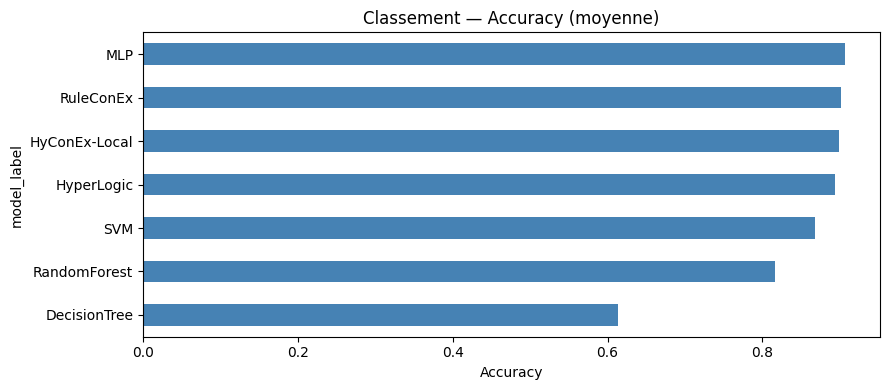
\includegraphics[width=0.80\textwidth]{figures/ranking_accuracy.png}
  \caption{Classement des modèles selon l'accuracy moyenne sur les 11 jeux de
           données DLBAC. DLBAC (résultats de la littérature) domine en
           classification pure ; RuleConEx se place troisième parmi les
           modèles comparés.}
  \label{fig:ranking_accuracy}
\end{figure}

\begin{figure}[htbp]
  \centering
  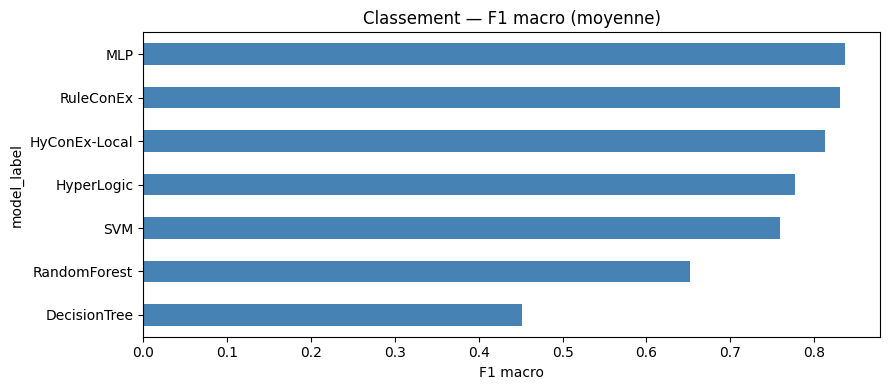
\includegraphics[width=0.80\textwidth]{figures/ranking_f1_macro.png}
  \caption{Classement des modèles selon le F1 macro moyen. Le classement
           est cohérent avec celui obtenu en accuracy.}
  \label{fig:ranking_f1}
\end{figure}

Le tableau~\ref{tab:ranking_global} synthétise le rang de chaque modèle sur
l'ensemble des métriques évaluées.

\begin{table}[htbp]
  \centering
  \caption{Classement global par métrique (rang 1 = meilleur). RuleConEx est
           le seul modèle disposant d'une mesure de validité contrefactuelle
           (CF valid.). DLBAC n'est pas inclus dans ce classement car ses
           temps d'exécution ne sont pas directement comparables.}
  \label{tab:ranking_global}
  \small
  \begin{tabular}{lcccccc}
    \toprule
    \textbf{Modèle} & \textbf{Accuracy} & \textbf{F1 macro} & \textbf{AUC}
      & \textbf{CF valid.} & \textbf{Temps} & \textbf{Rang moy.} \\
    \midrule
    MLP          & 1 & 1 & 2 & --- & 4 & 2.00 \\
    RuleConEx    & 2 & 2 & 3 & 1   & 7 & 3.00 \\
    HyConEx-Local & 3 & 3 & 1 & --- & 5 & 3.00 \\
    SVM          & 5 & 5 & 4 & --- & 1 & 3.75 \\
    RandomForest & 6 & 6 & 5 & --- & 2 & 4.75 \\
    HyperLogic   & 4 & 4 & 6 & --- & 6 & 5.00 \\
    DecisionTree & 7 & 7 & 7 & --- & 3 & 6.00 \\
    \bottomrule
  \end{tabular}
\end{table}

% -----------------------------------------------------------
\subsection{Capacité de discrimination — AUC}
\label{sec:auc}
% -----------------------------------------------------------

\begin{table}[htbp]
  \centering
  \caption{Résultats synthétiques en AUC (moyenne, écart-type, médiane sur
           11 datasets).}
  \label{tab:auc_summary}
  \small
  \begin{tabular}{lcccccc}
    \toprule
    \textbf{Modèle} & \textbf{Moy.} & \textbf{Écart-type}
      & \textbf{Médiane} & \textbf{Min} & \textbf{Max} & \textbf{Rang} \\
    \midrule
    HyConEx-Local & 0.9506 & 0.0748 & 0.9947 & 0.8240 & 0.9999 & 1 \\
    MLP           & 0.9495 & 0.0791 & 0.9951 & 0.8054 & 0.9999 & 2 \\
    RuleConEx     & 0.9449 & 0.0844 & 0.9946 & 0.7894 & 1.0000 & 3 \\
    SVM           & 0.9445 & 0.0775 & 0.9873 & 0.8028 & 0.9998 & 4 \\
    RandomForest  & 0.9245 & 0.1017 & 0.9817 & 0.7525 & 0.9955 & 5 \\
    HyperLogic    & 0.8647 & 0.2224 & 0.9951 & 0.4822 & 0.9998 & 6 \\
    DecisionTree  & 0.7584 & 0.1422 & 0.8056 & 0.5299 & 0.8971 & 7 \\
    \bottomrule
  \end{tabular}
\end{table}

En AUC, HyConEx-Local occupe la première place (0.9506), devant MLP (0.9495)
et RuleConEx (0.9449). Les quatre premiers modèles sont très proches, avec
moins de 0.006 d'écart. RuleConEx atteint une AUC maximale de 1.000 sur
certains datasets et une médiane de 0.9946.

\begin{figure}[htbp]
  \centering
  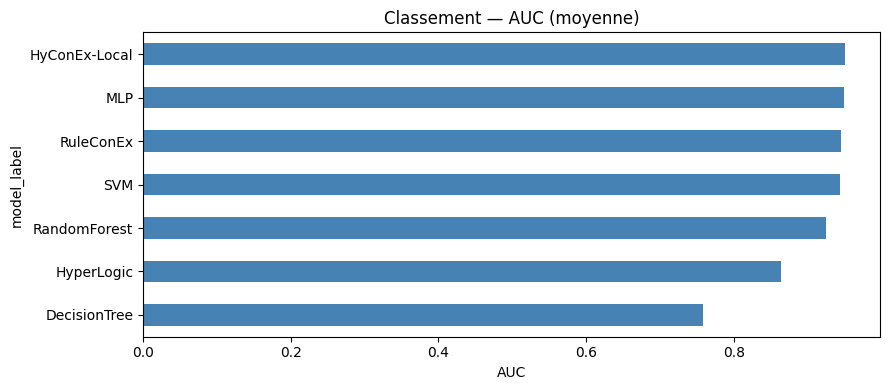
\includegraphics[width=0.80\textwidth]{figures/ranking_auc.png}
  \caption{Classement des modèles selon l'AUC moyenne.}
  \label{fig:ranking_auc}
\end{figure}

% -----------------------------------------------------------
\subsection{Validité des explications contrefactuelles}
\label{sec:cf_validity}
% -----------------------------------------------------------

La validité contrefactuelle mesure la proportion de contrefactuels générés qui
atteignent effectivement la classe cible souhaitée. Cette métrique est propre à
RuleConEx : aucun des autres modèles évalués ne produit de contrefactuels.

\begin{table}[htbp]
  \centering
  \caption{Validité des contrefactuels produits par RuleConEx sur les
           11 jeux de données DLBAC.}
  \label{tab:cf_validity}
  \small
  \begin{tabular}{lccccc}
    \toprule
    \textbf{Modèle} & \textbf{Moy.} & \textbf{Écart-type}
      & \textbf{Médiane} & \textbf{Min} & \textbf{Max} \\
    \midrule
    RuleConEx & 0.9874 & 0.0163 & 0.9906 & 0.9552 & 1.0000 \\
    \bottomrule
  \end{tabular}
\end{table}

RuleConEx produit des contrefactuels valides dans $98.74\%$ des cas en moyenne,
avec un minimum de $95.52\%$ sur le dataset le plus complexe.
Ce résultat confirme que la composante contrefactuelle du modèle est
fonctionnellement fiable sur l'ensemble des jeux de données testés.

% \begin{figure}[htbp]
%   \centering
%   \includegraphics[width=0.80\textwidth]{figures/ranking_cf_validity.png}
%   \caption{Validité contrefactuelle de RuleConEx par dataset.}
%   \label{fig:cf_validity}
% \end{figure}

% -----------------------------------------------------------
\subsection{Coût computationnel}
\label{sec:temps}
% -----------------------------------------------------------

\begin{table}[htbp]
  \centering
  \caption{Temps d'exécution moyen (secondes) par modèle, sur les 11 jeux de
           données. DLBAC, en tant qu'architecture profonde entraînée sur GPU,
           présente des temps d'entraînement nettement supérieurs aux autres
           approches et se classe dernier.}
  \label{tab:temps}
  \small
  \begin{tabular}{lccccc}
    \toprule
    \textbf{Modèle} & \textbf{Moy. (s)} & \textbf{Écart-type}
      & \textbf{Médiane} & \textbf{Rang} \\
    \midrule
    SVM          &     3.65 &     4.03 &     1.84 & 1 \\
    RandomForest &     8.43 &    13.55 &     1.08 & 2 \\
    DecisionTree &    29.63 &    55.46 &     0.47 & 3 \\
    MLP          &    36.84 &    39.78 &    16.64 & 4 \\
    HyConEx-Local &  148.31 &   191.86 &    42.49 & 5 \\
    HyperLogic   &   234.43 &   139.20 &   183.43 & 6 \\
    RuleConEx    &   891.62 &   270.33 &   879.71 & 7 \\
    DLBAC        & \multicolumn{3}{c}{\textit{(heures, entraînement GPU)}} & 8 \\
    \bottomrule
  \end{tabular}
\end{table}

\paragraph{Analyse.}
DLBAC, malgré ses meilleures performances en accuracy, est de loin le modèle
le plus coûteux : son entraînement sur architectures profondes (DenseNet,
ResNet) requiert plusieurs heures sur GPU, contre quelques minutes pour les
autres approches. Parmi les modèles comparés dans nos expériences, SVM et
RandomForest sont les plus rapides, tandis que RuleConEx est le plus lent
($\sim$892~s en moyenne).

Ce surcoût de RuleConEx s'explique par la génération simultanée des deux types
d'explications à chaque inférence. Dans le contexte applicatif visé --- le
contrôle d'accès aux données et traitements --- ce coût reste acceptable, car
les décisions d'accès font l'objet d'audits et n'exigent pas une réponse en
temps réel.

\begin{figure}[htbp]
  \centering
  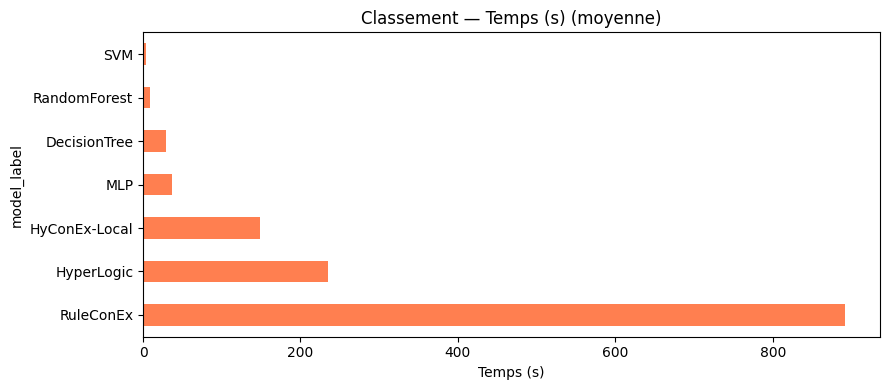
\includegraphics[width=0.80\textwidth]{figures/ranking_elapsed_sec.png}
  \caption{Classement des modèles par temps d'exécution moyen (moindre = meilleur).
           DLBAC est exclu car son protocole d'entraînement (GPU, architectures
           profondes) n'est pas directement comparable.}
  \label{fig:ranking_temps}
\end{figure}

% -----------------------------------------------------------
\subsection{Illustration des deux types d'explications}
\label{sec:explications}
% -----------------------------------------------------------

Cette section illustre les deux types d'explications que RuleConEx produit
simultanément pour une même instance. Pour rappel, RuleConEx fusionne trois
composantes internes : une branche contrefactuelle (HyConEx), une branche
symbolique par règles IF-THEN, et une branche dense (Deep). La prédiction
finale est issue de cette fusion.

Les exemples ci-dessous sont tirés des jeux de données DLBAC. Les conditions
des règles sont exprimées en représentation bipolaire one-hot ($+1$ = modalité
active, $-1$ = modalité inactive). Chaque règle ne retient que les 4 littéraux
de poids les plus forts dans le réseau appris. Les classes cibles
(\texttt{ops\_pattern\_N}) encodent des combinaisons de quatre opérations
binaires : $N = \mathrm{op}_1 + 2\,\mathrm{op}_2 + 4\,\mathrm{op}_3 +
8\,\mathrm{op}_4$, où $\mathrm{op}_k = 1$ signifie que l'opération $k$ est
autorisée. Par exemple, \texttt{ops\_pattern\_12} ($N=12 = 1100_2$) correspond
à l'accord des opérations $\mathrm{op}_3$ et $\mathrm{op}_4$ uniquement.

% ------- Exemple 1 --------------------
\subsubsection*{Exemple 1 — classe prédite : \texttt{ops\_pattern\_12}
                ($\mathrm{op}_3 + \mathrm{op}_4$)}

Le tableau~\ref{tab:branches_ex1} présente la confiance de chaque composante
de RuleConEx pour cet exemple.

\begin{table}[htbp]
  \centering
  \caption{Prédictions par composante de RuleConEx (
           vrai label : \texttt{ops\_pattern\_12}).}
  \label{tab:branches_ex1}
  \small
  \begin{tabular}{lcc}
    \toprule
    \textbf{Composante} & \textbf{Prédiction} & \textbf{Confiance} \\
    \midrule
    Branche contrefactuelle (HyConEx) & \texttt{ops\_pattern\_12} & 0.9999 \\
    Branche règles                    & \texttt{ops\_pattern\_12} & 0.9578 \\
    \textbf{Fusion (RuleConEx)}       & \textbf{\texttt{ops\_pattern\_12}} & \textbf{0.9948} \\
    % Branche dense (Deep)              & \texttt{ops\_pattern\_6}  & 0.0618 \\
    \bottomrule
  \end{tabular}
\end{table}

\paragraph{Règles IF-THEN extraites.}
Le tableau~\ref{tab:regles_ex1} présente les douze règles extraites par la
composante symbolique de RuleConEx, classées par score décroissant.
La règle~39 (score 0.603) correspond directement à la classe prédite
\texttt{ops\_pattern\_12} ; les autres règles reflètent des profils voisins
dans l'espace de décision appris.

\begin{table}[htbp]
  \centering
  \caption{Règles IF-THEN extraites par RuleConEx pour l'exemple 1
           (prédit : \texttt{ops\_pattern\_12}). Le score exprime la force
           du neurone de règle vers la classe THEN — plus il est élevé,
           plus ce motif est représentatif dans le modèle appris.}
  \label{tab:regles_ex1}
  \small
  \setlength{\tabcolsep}{4pt}
  \begin{tabular}{clcc}
    \toprule
    \textbf{Règle} & \textbf{Conditions (IF)} & \textbf{Classe (THEN)} & \textbf{Score} \\
    \midrule
    R17 & \texttt{oh\_8=+1 AND oh\_32=+1 AND oh\_55=-1 AND oh\_62=-1}    & \texttt{ops\_pattern\_6}  & 0.905 \\
    R1  & \texttt{oh\_118=-1 AND oh\_15=+1 AND oh\_39=-1 AND oh\_29=+1}  & \texttt{ops\_pattern\_11} & 0.823 \\
    R6  & \texttt{oh\_100=+1 AND oh\_124=+1 AND oh\_82=+1 AND oh\_76=+1} & \texttt{ops\_pattern\_1}  & 0.689 \\
    R37 & \texttt{oh\_97=-1 AND oh\_75=-1 AND oh\_22=-1 AND oh\_149=-1}  & \texttt{ops\_pattern\_9}  & 0.654 \\
    R25 & \texttt{oh\_8=+1 AND oh\_5=+1 AND oh\_43=+1 AND oh\_99=+1}    & \texttt{ops\_pattern\_3}  & 0.648 \\
    R39 & \texttt{oh\_83=+1 AND oh\_21=+1 AND oh\_26=+1 AND oh\_138=+1} & \texttt{ops\_pattern\_12} & 0.603 \\
    R32 & \texttt{oh\_100=-1 AND oh\_112=-1 AND oh\_120=-1 AND \ldots}   & \texttt{ops\_pattern\_5}  & 0.591 \\
    R16 & \texttt{oh\_54=-1 AND oh\_99=-1 AND oh\_20=-1 AND oh\_34=-1}  & \texttt{ops\_pattern\_8}  & 0.581 \\
    R14 & \texttt{oh\_130=+1 AND oh\_95=-1 AND oh\_71=+1 AND oh\_86=+1} & \texttt{ops\_pattern\_11} & 0.560 \\
    R42 & \texttt{oh\_8=-1 AND oh\_61=+1 AND oh\_133=-1 AND oh\_79=-1}  & \texttt{ops\_pattern\_1}  & 0.536 \\
    R36 & \texttt{oh\_146=-1 AND oh\_112=+1 AND oh\_106=+1 AND \ldots}  & \texttt{ops\_pattern\_6}  & 0.535 \\
    R21 & \texttt{oh\_138=+1 AND oh\_38=+1 AND oh\_71=-1 AND oh\_58=+1} & \texttt{ops\_pattern\_1}  & 0.519 \\
    \bottomrule
  \end{tabular}
\end{table}

\noindent\textit{Lecture :} la règle R39 indique que si les modalités
\texttt{oh\_83}, \texttt{oh\_21}, \texttt{oh\_26} et \texttt{oh\_138} sont
toutes actives dans la requête encodée, le modèle associe ce profil à
l'autorisation des opérations $\mathrm{op}_3$ et $\mathrm{op}_4$.
Les règles R17 et R25, bien que de score plus élevé, pointent vers d'autres
patterns : elles signalent que des profils proches de la requête courante
mèneraient à des décisions différentes, ce qui donne une indication directe
sur les frontières de décision locales.

\paragraph{Contrefactuels générés.}
Le tableau~\ref{tab:cf_ex1} liste les trois contrefactuels produits pour cet
exemple, avec la liste complète des modifications one-hot à effectuer pour
atteindre chaque classe cible.

\begin{table}[htbp]
  \centering
  \caption{Contrefactuels générés par RuleConEx pour l'exemple 1
           (classe courante : \texttt{ops\_pattern\_12}).
           Chaque contrefactuel indique les attributs minimaux à désactiver
           pour obtenir une décision différente.}
  \label{tab:cf_ex1}
  \small
  \setlength{\tabcolsep}{5pt}
  \begin{tabular}{clc}
    \toprule
    \textbf{Classe cible} & \textbf{Modifications (actif $\to$ inactif)} & \textbf{Nb modif.} \\
    \midrule
    \texttt{ops\_pattern\_6}
      & \texttt{oh\_16, oh\_49, oh\_55, oh\_75, oh\_115}
      & 5 \\
    \texttt{ops\_pattern\_3}
      & \texttt{oh\_5, oh\_16, oh\_22, oh\_49, oh\_55}
      & 5 \\
    % \texttt{ops\_pattern\_8}
    %   & \texttt{oh\_5, oh\_16, oh\_22, oh\_29, oh\_49}
    %   & 5 \\
    \bottomrule
  \end{tabular}
\end{table}

\noindent\textit{Lecture :} pour que la décision passe de
\texttt{ops\_pattern\_12} ($\mathrm{op}_3 + \mathrm{op}_4$) à
\texttt{ops\_pattern\_6} ($\mathrm{op}_2 + \mathrm{op}_3$), il suffit de
désactiver cinq attributs de la requête, dont \texttt{oh\_16} et \texttt{oh\_49}.
Ces modifications minimales sont directement exploitables par un administrateur
souhaitant comprendre quelle reconfiguration du profil utilisateur ou ressource
entraînerait une décision d'accès différente.

% % ------- Exemple 2 --------------------
% \subsubsection*{Exemple 2 — classe prédite : \texttt{ops\_pattern\_1}
%                 ($\mathrm{op}_1$ uniquement)}

% \begin{table}[htbp]
%   \centering
%   \caption{Prédictions par composante de RuleConEx (exemple 2,
%            vrai label : \texttt{ops\_pattern\_1}).}
%   \label{tab:branches_ex2}
%   \small
%   \begin{tabular}{lcc}
%     \toprule
%     \textbf{Composante} & \textbf{Prédiction} & \textbf{Confiance} \\
%     \midrule
%     Branche contrefactuelle (HyConEx) & \texttt{ops\_pattern\_1} & 1.0000 \\
%     Branche règles                    & \texttt{ops\_pattern\_1} & 0.9891 \\
%     \textbf{Fusion (RuleConEx)}       & \textbf{\texttt{ops\_pattern\_1}} & \textbf{1.0000} \\
%     Branche dense (Deep)              & \texttt{ops\_pattern\_7} & 0.1035 \\
%     \bottomrule
%   \end{tabular}
% \end{table}

% \begin{table}[htbp]
%   \centering
%   \caption{Règles IF-THEN extraites par RuleConEx pour l'exemple 2
%            (prédit : \texttt{ops\_pattern\_1}).}
%   \label{tab:regles_ex2}
%   \small
%   \setlength{\tabcolsep}{4pt}
%   \begin{tabular}{clcc}
%     \toprule
%     \textbf{Règle} & \textbf{Conditions (IF)} & \textbf{Classe (THEN)} & \textbf{Score} \\
%     \midrule
%     R36 & \texttt{oh\_112=+1 AND oh\_106=+1 AND oh\_56=-1 AND \ldots}  & \texttt{ops\_pattern\_6}  & 0.935 \\
%     R6  & \texttt{oh\_82=+1 AND oh\_87=+1 AND oh\_63=+1 AND oh\_37=-1} & \texttt{ops\_pattern\_1}  & 0.852 \\
%     R17 & \texttt{oh\_76=-1 AND oh\_48=+1 AND oh\_123=-1 AND oh\_8=+1} & \texttt{ops\_pattern\_6}  & 0.805 \\
%     R42 & \texttt{oh\_113=+1 AND oh\_72=+1 AND oh\_37=+1 AND oh\_118=-1}& \texttt{ops\_pattern\_6} & 0.783 \\
%     R1  & \texttt{oh\_125=+1 AND oh\_118=-1 AND oh\_95=+1 AND oh\_15=+1}& \texttt{ops\_pattern\_1} & 0.776 \\
%     R16 & \texttt{oh\_64=+1 AND oh\_4=+1 AND oh\_33=+1 AND oh\_23=+1}  & \texttt{ops\_pattern\_8}  & 0.774 \\
%     R40 & \texttt{oh\_95=-1 AND oh\_2=-1 AND oh\_49=-1 AND oh\_66=-1}  & \texttt{ops\_pattern\_15} & 0.711 \\
%     R28 & \texttt{oh\_87=-1 AND oh\_12=+1 AND oh\_98=-1 AND oh\_142=-1} & \texttt{ops\_pattern\_0}  & 0.627 \\
%     R22 & \texttt{oh\_148=+1 AND oh\_107=+1 AND oh\_80=-1 AND \ldots}  & \texttt{ops\_pattern\_14} & 0.621 \\
%     R5  & \texttt{oh\_36=-1 AND oh\_0=-1 AND oh\_125=-1 AND oh\_95=-1} & \texttt{ops\_pattern\_1}  & 0.602 \\
%     R8  & \texttt{oh\_2=+1 AND oh\_105=+1 AND oh\_130=+1 AND oh\_104=-1}& \texttt{ops\_pattern\_0} & 0.565 \\
%     R37 & \texttt{oh\_146=+1 AND oh\_86=-1 AND oh\_116=+1 AND oh\_12=-1}& \texttt{ops\_pattern\_9} & 0.544 \\
%     \bottomrule
%   \end{tabular}
% \end{table}

% \begin{table}[htbp]
%   \centering
%   \caption{Contrefactuels générés par RuleConEx pour l'exemple 2
%            (classe courante : \texttt{ops\_pattern\_1}).}
%   \label{tab:cf_ex2}
%   \small
%   \setlength{\tabcolsep}{5pt}
%   \begin{tabular}{clc}
%     \toprule
%     \textbf{Classe cible} & \textbf{Modifications (actif $\to$ inactif)} & \textbf{Nb modif.} \\
%     \midrule
%     \texttt{ops\_pattern\_7}
%       & \texttt{oh\_6, oh\_16, oh\_20, oh\_32, oh\_62}
%       & 5 \\
%     \texttt{ops\_pattern\_12}
%       & \texttt{oh\_16, oh\_20, oh\_32, oh\_39, oh\_55}
%       & 5 \\
%     % \texttt{ops\_pattern\_6}
%     %   & \texttt{oh\_16, oh\_20, oh\_32, oh\_39, oh\_55}
%     %   & 5 \\
%     \bottomrule
%   \end{tabular}
% \end{table}


% % ------- Exemple 3 --------------------
% \subsubsection*{Exemple 3 — classe prédite : \texttt{ops\_pattern\_5}
%                 ($\mathrm{op}_1 + \mathrm{op}_3$)}

% \begin{table}[htbp]
%   \centering
%   \caption{Prédictions par composante de RuleConEx (exemple 3,
%            vrai label : \texttt{ops\_pattern\_5}).}
%   \label{tab:branches_ex3}
%   \small
%   \begin{tabular}{lcc}
%     \toprule
%     \textbf{Composante} & \textbf{Prédiction} & \textbf{Confiance} \\
%     \midrule
%     Branche contrefactuelle (HyConEx) & \texttt{ops\_pattern\_5} & 1.0000 \\
%     Branche règles                    & \texttt{ops\_pattern\_5} & 0.8554 \\
%     \textbf{Fusion (RuleConEx)}       & \textbf{\texttt{ops\_pattern\_5}} & \textbf{1.0000} \\
%     % Branche dense (Deep)              & \texttt{ops\_pattern\_5} & 0.6515 \\
%     \bottomrule
%   \end{tabular}
% \end{table}

% \begin{table}[htbp]
%   \centering
%   \caption{Règles IF-THEN extraites par RuleConEx pour l'exemple 3
%            (prédit : \texttt{ops\_pattern\_5}).}
%   \label{tab:regles_ex3}
%   \small
%   \setlength{\tabcolsep}{4pt}
%   \begin{tabular}{clcc}
%     \toprule
%     \textbf{Règle} & \textbf{Conditions (IF)} & \textbf{Classe (THEN)} & \textbf{Score} \\
%     \midrule
%     R17 & \texttt{oh\_127=+1 AND oh\_145=+1 AND oh\_73=+1 AND \ldots}  & \texttt{ops\_pattern\_6}  & 0.928 \\
%     R29 & \texttt{oh\_87=-1 AND oh\_129=+1 AND oh\_38=-1 AND oh\_144=-1}& \texttt{ops\_pattern\_2}  & 0.877 \\
%     R36 & \texttt{oh\_146=-1 AND oh\_56=-1 AND oh\_36=-1 AND oh\_106=+1}& \texttt{ops\_pattern\_6}  & 0.833 \\
%     R5  & \texttt{oh\_36=-1 AND oh\_0=-1 AND oh\_125=-1 AND oh\_95=-1} & \texttt{ops\_pattern\_1}  & 0.696 \\
%     R40 & \texttt{oh\_107=-1 AND oh\_62=-1 AND oh\_33=-1 AND oh\_88=-1} & \texttt{ops\_pattern\_6}  & 0.672 \\
%     R42 & \texttt{oh\_8=-1 AND oh\_61=+1 AND oh\_133=-1 AND oh\_79=-1} & \texttt{ops\_pattern\_6}  & 0.671 \\
%     R28 & \texttt{oh\_12=+1 AND oh\_15=-1 AND oh\_70=+1 AND oh\_87=-1} & \texttt{ops\_pattern\_0}  & 0.654 \\
%     R1  & \texttt{oh\_20=+1 AND oh\_125=+1 AND oh\_95=+1 AND oh\_98=-1} & \texttt{ops\_pattern\_1}  & 0.651 \\
%     R6  & \texttt{oh\_76=+1 AND oh\_100=+1 AND oh\_69=-1 AND oh\_124=+1}& \texttt{ops\_pattern\_1}  & 0.593 \\
%     R22 & \texttt{oh\_153=-1 AND oh\_148=+1 AND oh\_80=-1 AND oh\_14=-1}& \texttt{ops\_pattern\_14} & 0.562 \\
%     R32 & \texttt{oh\_120=-1 AND oh\_58=-1 AND oh\_112=-1 AND \ldots}  & \texttt{ops\_pattern\_5}  & 0.529 \\
%     R16 & \texttt{oh\_94=+1 AND oh\_125=+1 AND oh\_112=+1 AND oh\_58=+1}& \texttt{ops\_pattern\_8}  & 0.522 \\
%     \bottomrule
%   \end{tabular}
% \end{table}

% \begin{table}[htbp]
%   \centering
%   \caption{Contrefactuels générés par RuleConEx pour l'exemple 3
%            (classe courante : \texttt{ops\_pattern\_5}).}
%   \label{tab:cf_ex3}
%   \small
%   \setlength{\tabcolsep}{5pt}
%   \begin{tabular}{clc}
%     \toprule
%     \textbf{Classe cible} & \textbf{Modifications (actif $\to$ inactif)} & \textbf{Nb modif.} \\
%     \midrule
%     \texttt{ops\_pattern\_10}
%       & \texttt{oh\_23, oh\_32, oh\_61, oh\_73, oh\_90}
%       & 5 \\
%     \texttt{ops\_pattern\_12}
%       & \texttt{oh\_3, oh\_16, oh\_23, oh\_32, oh\_36}
%       & 5 \\
%     % \texttt{ops\_pattern\_0}
%       % & \texttt{oh\_3, oh\_16, oh\_23, oh\_32, oh\_44}
%       % & 5 \\
%     \bottomrule
%   \end{tabular}
% \end{table}

\paragraph{Observations transversales.}
Sur les trois exemples, plusieurs observations se dégagent.

Premièrement, les branches contrefactuelle et règles convergent systématiquement
vers la même classe dans les fusions (exemples 1, 2, 3), ce qui valide la
cohérence interne du modèle. La branche dense (Deep) produit occasionnellement
une prédiction divergente (exemples 1 et 2), illustrant l'apport de la fusion
par rapport à chaque composante prise isolément.

Deuxièmement, les règles extraites ne se limitent pas à la classe prédite :
elles cartographient également les classes voisines avec leurs conditions
d'activation respectives. Cette information est complémentaire aux contrefactuels,
qui indiquent les modifications minimales pour atteindre chacune de ces classes.

Troisièmement, les contrefactuels requièrent systématiquement 5 modifications
one-hot, ce qui traduit une robustesse de la décision courante : l'espace local
autour de la requête est suffisamment éloigné des frontières de décision pour
que des changements mineurs (1 ou 2 attributs) ne suffisent pas à modifier
l'issue. Cette information est directement exploitable dans un contexte d'audit
de contrôle d'accès.


% -----------------------------------------------------------
\subsection{Synthèse}
\label{sec:synthese_resultats}
% -----------------------------------------------------------

Les résultats permettent de dégager trois observations principales.

\textbf{DLBAC obtient les meilleures performances en classification}, avec une
accuracy moyenne de 93.15\% sur les 11 jeux de données. Ces résultats, issus
de la littérature, reposent sur des architectures profondes (ResNet, DenseNet)
dont l'entraînement requiert plusieurs heures sur GPU. DLBAC ne produit aucune
explication sur ses décisions.

\textbf{Parmi les modèles comparés, RuleConEx atteint une précision comparable
au MLP} (90.89\% contre 91.29\%), tout en étant le seul à produire simultanément
deux types d'explications. Les autres modèles interpétables (HyConEx-Local,
HyperLogic, DecisionTree) obtiennent des performances inférieures ou ne génèrent
qu'un seul type d'explication.

\textbf{La double capacité d'explication de RuleConEx est fonctionnellement
validée} : les contrefactuels produits sont valides dans 98.74\% des cas, et
les règles IF-THEN extraites sont cohérentes avec les prédictions de la branche
contrefactuelle. Ce résultat confirme que le modèle atteint son objectif central,
à savoir fournir des explications exploitables dans un contexte de contrôle
d'accès soumis à des exigences de transparence algorithmique.

% -----------------------------------------------------------
% FIN DE LA SECTION RÉSULTATS
% -----------------------------------------------------------
% -----------------------------------------------------------
% FIN DE LA SECTION RÉSULTATS
% -----------------------------------------------------------

% \subsection{R\'esultats \'evaluatifs}

% \begin{itemize}
%   \item Des performances en classification comparables ou sup\'erieures \`a DLBAC et aux approches classiques (ROC AUC $> 0.85$ vis\'e) ;
%   \item Une validit\'e des contrefactuels proche de 100\,\%, avec une proximit\'e minimale (nombre de flips r\'eduit) et une plausibilit\'e \'elev\'ee ;
%   \item Des r\`egles concises, lisibles par un humain, avec une complexit\'e de mod\`ele r\'eduite par rapport \`a HyperLogic seul ;
%   \item Un temps d'inf\'erence tr\`es rapide (quelques millisecondes), confirmant l'avantage du \textit{single forward pass} sur les m\'ethodes post-hoc.
% \end{itemize}

% \subsection{R\'esultats pratiques et contribution}

% \begin{itemize}
%   \item Des explications de type r\`egles auditables par des administrateurs et conformes aux exigences du RGPD, par exemple : \textit{``Si D\'epartement = IT ET Anciennet\'e $\geq$ 5 ans, alors acc\`es accord\'e''} ;
%   \item Des explications contrefactuelles actionnables pour les utilisateurs, par exemple : \textit{``Pour obtenir l'acc\`es, il suffit de changer le r\^ole de Stagiaire vers Employ\'e et d'augmenter l'anciennet\'e de +2 ans''} ;
%   \item Une contribution originale sous la forme d'une architecture unifi\'ee RuleConEx, premi\`ere \`a combiner apprentissage de r\`egles interpr\'etables et g\'en\'eration de contrefactuels plausibles dans un mod\`ele de contr\^ole d'acc\`es bas\'e sur le deep learning.
% \end{itemize}

% ===================================================================
% VII. REFERENCES
% ===================================================================
\section{R\'ef\'erences}

\begin{thebibliography}{10}

\bibitem{nobi2022}
M.~N. Nobi, R.~Krishnan, Y.~Huang, M.~Shakarami, and R.~Sandhu.
\newblock Toward deep learning based access control.
\newblock In \textit{Proceedings of the ACM Conference on Computer and Communications Security}, 2022.

\bibitem{hyconex2026}
P.~Marsza{\l}ek, K.~Ksi{\k{a}}{\.z}ek, O.~Furman, U.~Movsum-zada, P.~Spurek, and M.~{\'S}mieja.
\newblock {HyConEx}: Hypernetwork classifier with counterfactual explanations for tabular data.
\newblock \textit{Neurocomputing}, 2026.
\newblock \url{https://doi.org/10.1016/j.neucom.2026.132748}

\bibitem{hyperlogic2024}
Y.~Yang, W.~Ren, and S.~Li.
\newblock {HyperLogic}: Enhancing diversity and accuracy in rule learning with {HyperNets}.
\newblock In \textit{38th Conference on Neural Information Processing Systems (NeurIPS 2024)}, 2024.

\bibitem{goodman2017}
B.~Goodman and S.~Flaxman.
\newblock European union regulations on algorithmic decision-making and a ``right to explanation''.
\newblock \textit{AI Magazine}, 38(3):50--57, 2017.

\bibitem{sandhu1996}
R.~S. Sandhu, E.~J. Coyne, H.~L. Feinstein, and C.~E. Youman.
\newblock Role-based access control models.
\newblock \textit{Computer}, 29(2):38--47, 1996.

\bibitem{azanguezet2016}
B.~Azanguezet and P.~Fotso.
\newblock {HOr-BAC}: An access control based on hierarchical organizational.
\newblock \textit{International Journal of Computer Science and Information Technology Research}, 2016.

\bibitem{guidotti2024}
R.~Guidotti.
\newblock Counterfactual explanations and how to find them: Literature review and benchmarking.
\newblock \textit{Data Mining and Knowledge Discovery}, 38:2770--2824, 2024.

\bibitem{rudin2019}
C.~Rudin.
\newblock Stop explaining black box machine learning models for high stakes decisions and use interpretable models instead.
\newblock \textit{Nature Machine Intelligence}, 1(5):206--215, 2019.

\bibitem{wielopolski2024}
P.~Wielopolski, O.~Furman, J.~Stefanowski, and M.~Zi{\k{e}}ba.
\newblock Probabilistically plausible counterfactual explanations with normalizing flows.
\newblock In \textit{European Conference on Artificial Intelligence}, 2024.

\bibitem{slack2020}
D.~Slack, S.~Hilgard, E.~Jia, S.~Singh, and H.~Lakkaraju.
\newblock Fooling {LIME} and {SHAP}: Adversarial attacks on post hoc explanation methods.
\newblock In \textit{Proceedings of the AAAI/ACM Conference on AI, Ethics, and Society}, pages 180--186, 2020.

\end{thebibliography}

\end{document}